\documentclass[letterpaper,10pt, draftclsnofoot,onecolumn]{IEEEtran}
\usepackage[top=0.75in, bottom=0.75in, left=0.75in, right=0.75in]{geometry}
\usepackage[english]{babel}
\usepackage{amsmath}
\usepackage{amssymb,amsfonts,textcomp}
\usepackage{color}
\usepackage{array}
\usepackage{supertabular}
\usepackage{hhline}
\usepackage{hyperref}
\usepackage{float}
\usepackage{type1cm}
\hypersetup{pdftex, colorlinks=true, linkcolor=black, citecolor=blue, filecolor=black, urlcolor=black, pdftitle=SYSTEMS AND SOFTWARE REQUIREMENTS SPECIFICATION (SSRS) TEMPLATE}
\usepackage[pdftex]{graphicx}
% Outline numbering
\setcounter{secnumdepth}{5}

\makeatletter
\newcommand\arraybslash{\let\\\@arraycr}
\makeatother
% Page layout (geometry)
\usepackage{geometry}
\geometry{textheight=8.5in, textwidth=6in}
% Footnote rule
\setlength{\skip\footins}{0.0469in}









% footnotes configuration
\makeatletter
\renewcommand\thefootnote{\arabic{footnote}}
\makeatother
\title {The Client Requirements Document of App and website for Health Sciences Careers in Oregon }
\author{Zixuan Feng
	   Jason Ye
	   David Corbelli }
\date{October, 2016}
\begin{document}

\begin{flushleft}

   
        \Huge\textbf{SOFTWARE REQUIREMENTS\\ SPECIFICATION}\\
        \vspace{1.9cm}
        \large Sponsor \\
      	\LARGE\textbf {Oregon State Department of Education}\\
        \vspace{1.2cm}
        \LARGE\textbf {Prepared by Capstone 41}\\
        \vspace{1.9cm}
		\abstract{~The application and website for Oregon science is a guide for middle school and high school level students to learn about health science careers. 
        Between an application and website, the service shall provide information as exploration tool for students looking for future careers in health science. 
        Due to the many fields under the classification of health and science, it may be difficult for a student beginning to take an interest in the subject to find the proper path they're looking for.
        As a development team we will focus on developing an exploratory website and then develop corresponding applications for Android OS. 
        Through our platform, students will explore pathways and careers in health and science.}
    
\end{flushleft}


\begin{flushleft}
\clearpage{\selectlanguage{english}\bfseries\color{black}

\par}
\end{flushleft}

%%%%%%%%%%%%%%%%%%%%%%%%%%%%%%%%Head page%%%%%%%%%%%%%%%%%%%%%%%%%%%%%%%%%%%%%%%%
\vspace{-1.5cm}
\setcounter{tocdepth}{9}
\renewcommand\contentsname{}
\tableofcontents

\clearpage{\selectlanguage{english}\color{black}


\section[Introduction]{\selectlanguage{english}\color{black}
Introduction}


\subsection[Purpose]{\selectlanguage{english}\color{black}Purpose}
{\selectlanguage{english}\color{black}\normalsize
\noindent{This document introduces information, process, and user characters relevant to this project. This document will explain details of the product including the product perspective and necessary functions, as well as illustrate its benefit to users.
}


\subsection[Scope]{\selectlanguage{english}\color{black}
Scope}
\noindent{This project consists of creating a website and mobile application that will provide accurate and updated information based upon information from the Oregon Department of Education. The project will be completed by May, 2016. Modules of the website and app will include information about career pathways, administration tools, and a way to help student.
}
{\selectlanguage{english}\color{black}\normalsize


}

\subsection[Overview]{\selectlanguage{english}\color{black}
Overview}
{\selectlanguage{english}\color{black}\normalsize\noindent

\noindent{The remainder of this document describes the overall of the functionality of the product. It will describe the perspective and functions, introduce user characteristics, project constraints, assumptions and dependencies, as well as the apportioning of requirements.}onecolumn 


%%%%%%%%%%%%%%%%%%%Introduction Section 1 %%%%%%%%%%%%%%%%%%%%%%%%%%%%%%%%%%%%%
\clearpage{\selectlanguage{english}\color{black}
\section[Overall Description]{\selectlanguage{english}\color{black}
Overall Description}


\subsection[Product Perspective]{\selectlanguage{english}\color{black}
Product Perspective}
{\selectlanguage{english}\color{black}\normalsize\noindent
{The website displays pages containing information pertaining to the separate branches of health science careers; each page may also provide links to pages with more specific fields. 
There is also navigation supported for pages including educator tools, workforce partners, and education centers. 
The majority of the website information will be stored in a database for easy manipulation. 
Additionally a mobile companion application will be available based upon a mobile web browser to provide an alternative viewing platform.}



\subsection[Product Functions]{\selectlanguage{english}\color{black}
Product Functions}
{\selectlanguage{english}\color{black}\normalsize\noindent
The website designed for Health and Science Careers in Oregon allows users to interact through both web browsers and mobile devices. 
Users are able to navigate through a series of informative pages to learn about the different fields within health sciences. 
Alternatively, users may also use a search bar to view pages that include desired keywords. 
The website is also designed for mobile viewing and includes the same features as the desktop site.}


\subsection[User Characteristics]{\selectlanguage{english}\color{black}
User Characteristics}
{\selectlanguage{english}\color{black}\normalsize\noindent
The website is focused for middle and high school level students. 
Students at this level begin to choose their future career paths and to some it is still unclear how to start their goals and what requirements they need to fulfill. 
This website is meant to bridge this gap and provide an opportunity for exploration and learning. }

\subsection[Constraints]{\selectlanguage{english}\color{black}
Constraints}
{\selectlanguage{english}\color{black}\normalsize\noindent
The application for mobile devices may be constrained by differences in mobile devices based on display size. 
There exist many different display sizes and aspect ratios to take into account. 
Network connection is also a constraining factor as information is pulled not only from a web server, but also from a database. 
Should connection be poor, the required time for a page to load may vary, along with the time it takes to query the database.}


\subsection[Assumptions and Dependencies]{\selectlanguage{english}\color{black}
Assumptions and Dependencies}
{\selectlanguage{english}\color{black}\normalsize\noindent
Detailed information concerning careers in health sciences is provided by the Oregon Department of Education.
Additionally, a secure hosting server and database for the final product will be provided by the Oregon Department of Education. 
Publishing of the mobile application will also be managed by the Oregon Department of Education.}



\subsection[Additional Requirements]{\selectlanguage{english}\color{black}
Additional Requirements}
{\selectlanguage{english}\color{black}\normalsize\noindent
The site will include an additional backend page and documentation for updating pages and the database with new information. } 





\subsection[Apportionment of Requirements]{\selectlanguage{english}\color{black}
Apportionment of Requirements}\noindent
The project time frame is as detailed by the following Gantt chart.

\begin{figure}[H]
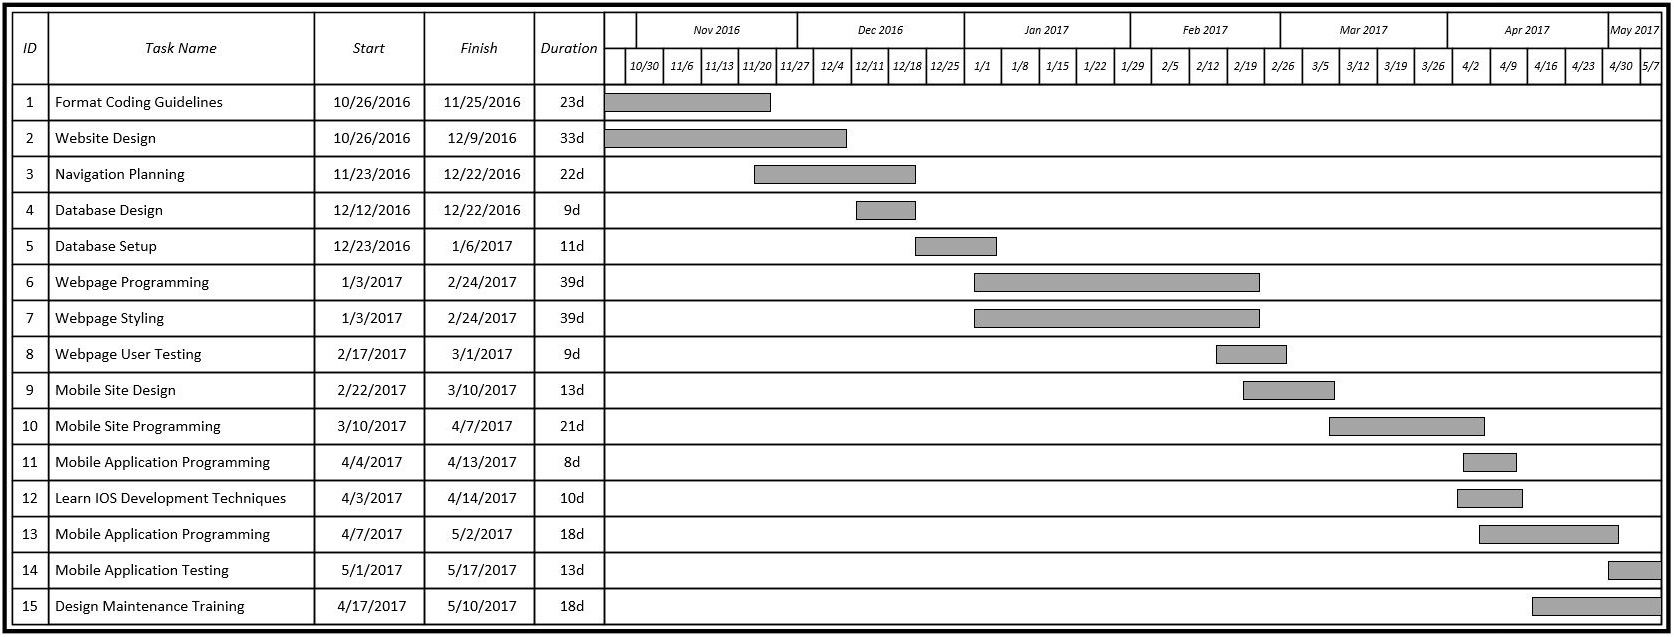
\includegraphics[scale=0.5]{GANTTv2.JPG}
\end{figure}


 
 
 \clearpage\setcounter{page}{1}


\bigskip

{\centering\selectlanguage{english}\color{black}
The Client Requirements Document of App and website for Health Sciences Careers in Oregon
\par}


\bigskip

{\centering\selectlanguage{english}\bfseries\color{black}
Version 1.0, 2016-10-26
\par}


 \vspace{2cm}
\noindent 
Zixuan Feng \\
Email: fengzi@oregonstate.edu\\
Address: 1148 Kelley Engineering Center, 2500 NW Monroe Ave, Corvallis, OR 97331\\


 \vspace{1cm}
\noindent 
Jason Ye \\
Email:yeja@oregonstate.edu\\
Address: 1148 Kelley Engineering Center, 2500 NW Monroe Ave, Corvallis, OR 97331\\


 \vspace{1cm}
\noindent 
David Corbelli \\
Email:Corbelld@oregonstate.edu\\
Address: 1148 Kelley Engineering Center, 2500 NW Monroe Ave, Corvallis, OR 97331\\

\clearpage\setcounter{page}{1}


\LARGE Signatures 
\par}
\vspace{1cm}
Art Witkowski	

\vspace{3cm}

David Corbelli
\vspace{3cm}

Jason Ye
\vspace{3cm}

Zixuan Feng
\end{document}